The increasing interest in lithium-ion batteries stems from their potential to offer efficient energy storage and contribute to environmental sustainability. Not only are LIBs widely employed in portable electronics like computers and cell phones, but they have also become integral to the power systems of electric or hybrid vehicles. The increasing popularity of LIBs in these applications can be attributed to their outstanding performance and high energy density \cite{kang2020binder}. Moreover, LIBs dominate the battery market for portable electronics, owing to inherent advantages such as high specific capacity and voltage, absence of memory effect, excellent cycling performance, minimal self-discharge, and a wide temperature range of operation \cite{zubi2018lithium}.

\vspace{5mm}

\begin{table}[ht]
    \centering
        \begin{footnotesize}
            \begin{tabular}{|p{7mm} p{22mm} p{113mm}|}
                \hline
                \rowcolor{bluepoli!40}
                \textbf{No.} & \textbf{Date} & \textbf{Accidents Replay}\T\B \\
                \hline \hline
                1 & Mar 2010 & Two iPod Nano music players overheated and caught fire, Japan\T\B\\
                2 & Apr 2010 & Acer recalled 2700 laptop batteries, as Dell, Apple, Toshiba, Lenovo and Sony did in 2006\T\B\\
                3 & Apr 2011 & EV taxi caught fire, Hangzhou, China\T\B\\
                4 & Jan-Dec 2013 & Three fire accidents of Boeing 747, happened in Boston America, Takamatsu, Tokyo Japan, respectively\T\B\\
                5 & Oct-Nov 2013 & 6 Tesla Model S EV cars caught fire\T\B\\
                6 & Apr 2015 & EV bus caught fire during charge, Shenzhen, China\T\B\\
                7 & May 2016 & The storage room of the LIB caught explosion, Jiangsu, China\T\B\\
                8 & Aug 2016 & Samsung Note 7 smart phone explosion\T\B\\
                9 & May 2017 & Panasonic announced to recall over 270 thousand LIBs\T\B\\
                10 & Oct 2017 & EV car caught fire, Austria\T\B\\
                11 & Jan 2018 & Tesla Model S EV car self-ignited, China\T\B\\
                12 & Jul 2018 & 4 MW/12 MWh energy storage system (ESS) caught fire and explosion, Korea\T\B\\
                13 & Jul 2018 & Electric scooter caught fire and explosion during charging, China\T\B\\
                \hline
                \end{tabular}
                \\[10pt]
                \caption[Lithium-ion battery accidents]{Lithium-ion battery fire and explosion accidents in the past few years. Source: Wang (2019) \cite{wang2019review}.}
                \label{table:accidents}
        \end{footnotesize}
\end{table}


Despite these merits, the broader expansion of the LIB market, especially in electric vehicles, faces significant challenges due to safety concerns \cite{love2018innovating,schipper2016recent,feng2018thermal}. Recent years have witnessed numerous recalls of LIBs, prompted by incidents of explosions and fires (Table \ref{table:accidents}), leading to substantial economic repercussions in related market sectors and tarnishing the reputation of LIBs \cite{chen2021review,balakrishnan2006safety}. As a result, there is a growing emphasis on addressing LIB safety issues, with the development of numerous safety strategies aimed at mitigating the risks associated with these batteries.

\section{Safety Standards}
\label{sec:safety-standards}

Safety standards and corresponding assessments have been established to analyze battery performance and key factors, aligning with the necessary safety requisites. The stringent and rigorous battery safety tests are designed to minimize the likelihood of safety issues in routine working conditions and ensure that batteries available on the market are of sufficient quality for intended purposes. Thanks to these measures, contemporary LIBs exhibit a significantly enhanced safety profile compared to their predecessors. Nonetheless, ongoing advancements are imperative to further improve battery safety standards \cite{chen2021review}.

Hence, various international safety organizations regulate battery safety, and governments of different countries have formulated safety standards in accordance with national requirements and conditions and have gradually improved the safety standards of lithium-ion batteries. Academics and industrial groups have also carried out extensive research on battery safety.

Most countries and international organizations have developed LIB-safety oriented standards, which include:
\begin{enumerate}
    \item Chinese standard GB/T 31485 \cite{};
    \item Society of Automotive Engineers (SAE) standard 2464 \cite{};
    \item International Electrotechnical Commission (IEC) standard IEC62133 Edition 2.0 \cite{};
    \item United Nations (UN) standard UN38.3 \cite{};
    \item Japanese Industrial Standard (JIS) C8714 \cite{};
    \item Underwriters Laboratories (UL) standard UL2580 Edition 2.0 \cite{};
    \item International Standardization Organization (ISO) standard
    ISO 16750-2 \cite{};
\end{enumerate}

Since the various safety test standars apply different methodologies, a summary of some test requirements and comparisons of five test items are presented in Table \ref{table:standards}.

\begin{table}[ht]
    \centering
        \begin{scriptsize}
            \begin{tabular}{|p{26mm} p{26mm} p{26mm} p{26mm} p{26mm}|}
                \hline
                \rowcolor{bluepoli!40}
                 & \textbf{GB/T31485} & \textbf{IEC62133} & \textbf{UL2580} & \textbf{SAE J2464}\T\B \\
                \hline \hline
                \textbf{Heating} &  &  &  & \T\B\\
                \textbf{Short-circuit} &  &  &  & \T\B\\
                \textbf{Overcharge} &  &  &  & \T\B\\
                \textbf{Over-discharge} &  &  &  & \T\B\\
                \textbf{Nail penetration} &  &  &  & \T\B\\
                \hline
                \end{tabular}
                \\[10pt]
                \caption[Testing standards coparison]{Testing standards comparison of selected items. $\varphi$ represents the nail diameter. Source: Chen (2021) \cite{chen2021review}.}
                \label{table:standards}
        \end{scriptsize}
\end{table}



\subsection{Safety Tests}
\label{sec:safety-tests}
Analysis of the presence of various LIB defects and shortcomings can help to define specific LIB safety issues or hazards. Extensive testing uncovers these issues to assist efforts to ensure that future generations of batteries are safer and more reliable. In a safety test possible trigger modes are simplified so batteries thermal runaway characteristics are measurable in the laboratory. Laboratory environment test conditions must generally be more stringent than "real-world" conditions to ensure safety during actual use. For example, batteries being tested have to be maintained at a 100\% state of charge (SOC). The three principles of operability, repeatability and reproducibility should be met in the process of formulating a safety standard. 

Here follows a brief description of the main safety tests used to examine key LIB properties:

\begin{itemize}
    \item[--] \textbf{Overcharge tests} are intended to assess overcharge/over-discharge processes that occur in a cell when the charge and discharge process is out of control. According to the IEC standard test, the cell is first discharged to 3.0 V, and then is charged under 10 V. If the battery does not combust or explode during or after the test it is considered safe, its materials (electrolyte, active electrode materials, separators etc.) are regarded as having adequate properties, and the structural design is deemed satisfactory. The safety performance under overcharge is closely related to the charge rate, so overcharging is performed at different rates to establish at which extreme rate and voltage failure occurs.
    \item[--] \textbf{Heating tests} assess the thermal runaway caused by a battery being heated due to local overheating, and the subsequent thermal runaway expansion. Heating is used to analyze LIBs' thermal stability and heat distribution to ensure they have sufficiently efficient heat management and capability to forecast potential hazards. The results are then used to assess how thermal abuse consequences can be alleviated. Specifically, data obtained from hot box experiments are used to simulate their thermal characteristics, and distributions of internal and external temperatures, then assess possible improvements in their design, materials, cooling systems, etc.
    \item[--] \textbf{Short circuit tests}
    \begin{itemize}
        \item \textbf{External short circuit tests} assess the short circuiting that is caused by external electrical connections of battery poles under abnormal conditions. \textbf{Qua manca la prosecuzione della descrizione!}
        \item \textbf{Internal short circuit tests} assess the short circuiting that is caused by internal electrical connections of battery poles under abnormal conditions. \textbf{Qua manca la prosecuzione della descrizione!}
        \item \textbf{Nail penetration tests} assess effects of a battery short circuiting if the separator is penetrated by impurities. \textbf{Qua manca la prosecuzione della descrizione!}
    \end{itemize}
\end{itemize}

\subsection{Hazard level}
\label{sec:hazard-level}
In evaluations of batteries' safety condition based on results of the above abuse tests, the EUCAR Hazard Levels and the associated criteria that are widely applied. Typically, hazard levels of Electrical Energy Storage System (EESS) devices according to their responses to abuse conditions are assigned by EUCAR and presented in Table \ref{table:eucar}. Manufacturers and integrators may find it helpful and useful to take these levels into consideration when evaluating a given EESS design's abuse response.

\begin{table}[ht]
    \centering
        \begin{footnotesize}
            \begin{tabular}{|p{13mm} p{28mm} p{102mm}|}
                \hline
                \rowcolor{bluepoli!40}
                \textbf{Hazard Level} & \textbf{Description} & \textbf{Classification Criteria \& Effect}\T\B \\
                \hline \hline
                0 & No effect & No effect. No loss of functionality.\T\B\\
                \hline
                1 & Passive protection activated & No defect; no leakage; no venting, fire or flame; no rupture; no explosion; no exotermic reaction or thermal runaway. Cell reversibly damaged. Repair of protection device needed.\T\B\\
                \hline
                2 & Defect/Damage & No leakage; no venting, fire or flame; no rupture; no explosion; no exotermic reaction or thermal runaway. Cell irreversibly damaged. Repair needed.\T\B\\
                \hline
                3 & Leakage & No venting, fire or flame; no rupture; no explosion.\\
                & ($\Delta$ mass $<$ 50\%) & Weight loss $<$ 50\% of electrolyte weight (electrolyte = solvent + salt).\T\B\\
                \hline
                4 & Venting & No fire or flame; no rupture; no explosion.\\
                & ($\Delta$ mass $\geq$ 50\%) & Weight loss $\geq$ 50\% of electrolyte weight (electrolyte = solvent + salt).\T\B\\
                \hline
                5 & Fire or Flame & No rupture; no explosion (i.e. no flying parts).\T\B\\
                \hline
                6 & Rupture & No explosion, but flying parts of the active mass.\T\B\\
                \hline
                7 & Explosion & Explosion (i.e. disintegration of the cell).\T\B\\
                \hline
                \end{tabular}
                \\[10pt]
                \caption[EUCAR hazard levels]{EUCAR hazard levels and associated criteria. Source: EUCAR (2019) \cite{eucar2019}.}
                \label{table:eucar}
        \end{footnotesize}
\end{table}

\section{Thermal Runaway}
\label{sec:thermal-runaway}

\begin{figure}[ht]
    \centering
    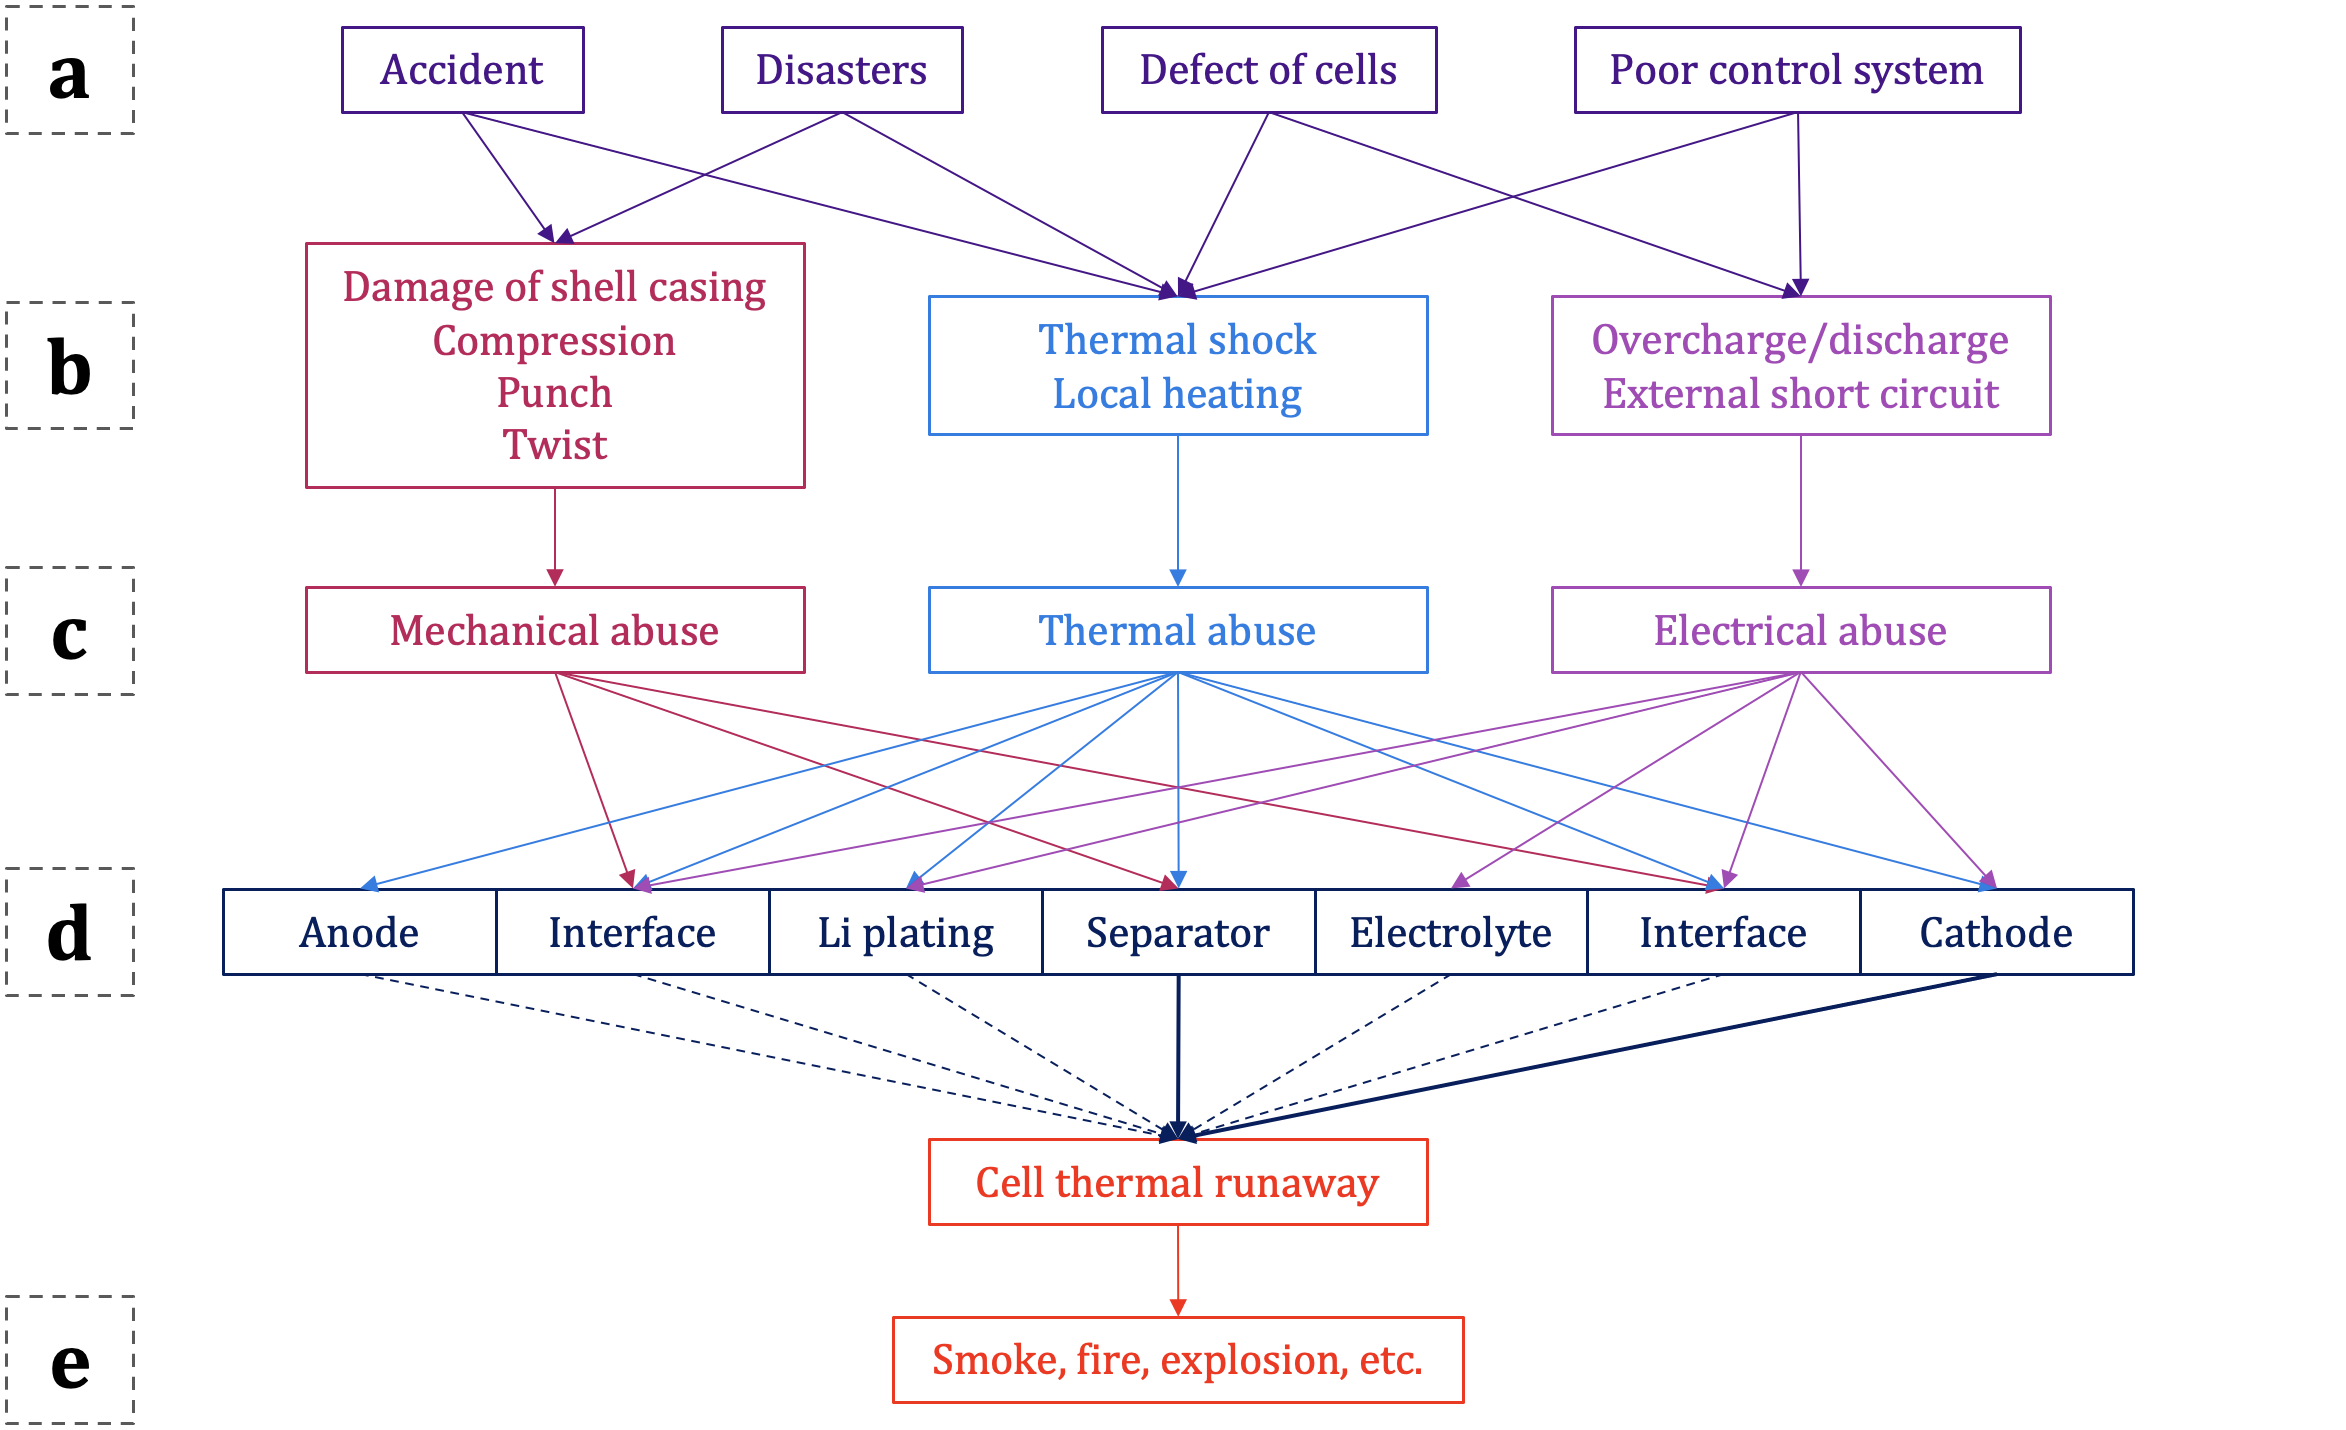
\includegraphics[width=0.9\textwidth]{Images/Chapter1/tr-graph.png}
    \caption[Schematic of the causes of lithium-ion battery thermal runaway]{Schematic of the causes of lithium-ion battery thermal runaway. Breakage of the separator and the oxygen evolution from the cathode side are the root causes to batteries' thermal runaway (as shown by the solid lines). Source: Chen (2020) \cite{chen2021review}.}
    \label{fig:tr-graph}
\end{figure}

\textbf{Queste frasi sono copiaincollate da} \texttt{chen2021review}\textbf{, quindi sono da riscrivere.}

Rising battery temperature would trigger other undesirable parasitic reactions, causing thermal runaway, where battery heat generation cannot be controlled \cite{wang2012thermal}.
During mechanical (damage to shell casing, compression, punching, and twisting of cells), electrical (overcharge/discharge and short circuit), and thermal abuse (thermal shock and local heating) situations, which could occur during accidents, thermal runaway will occur even quicker \cite{guo2010three,kim2007three,lamb2014evaluation}. Understanding LIB performance in unsafe conditions is critical, therefore, for the pro- duction of safer cells.

In the normal voltage and temperature range, only Li+ shuttle occurs in the electrolyte during the insertion/extraction cycles at the cathode and anode. At high-temperature and high-voltage conditions, the electrochemical reactions become more complex, including decomposition of the solid electrolyte interface (SEI) film, oxygen release at the cathode side, and additional electrolyte/electrode parasitic side reactions \cite{maleki1999thermal}. SEI film decomposition and interfacial reactions initially accelerate the temperature increase, thereby increasing risks of oxygen release from the active cathode materials. These reactions eventually lead to LIB thermal runaway, which causes battery rupture and explosion due to the reaction of hot flammable gases from the battery with the ambient oxygen \cite{finegan2016investigating}.

There are five types of causes for this phenomenon, which are illustrated in Fig. 2. The first type is uncontrollable internal heat generation, which causes oxygen release from the cathode material, leading to numerous side reactions [[37,53]]. In the second type, separator defects (due to thermally-induced shrinkage or mechan- ical damage) create short circuits in the battery and rapid discharge of the energy stored in it [[54]], accompanied by undesirable chemical chain reactions and release of massive amounts of heat. The third type is electrical abuse [[55]]. Electrolyte decomposition, especially in a high state of charge (SOC), occurs at the cathode interface. This leads to heat accumulation and consequently release of oxygen from the cathode and damage to the separator. The fourth type consists of electrochemical side reactions caused by local thermal abuse. If the heat generated during normal LIB operations cannot be dissipated quickly enough, the separator in that specific place will shrink or rupture [[41,56]]. The fifth type occurs during mechanical battery damage, which causes short circuits and/or air to penetrate the battery [[57]]. The main causes of battery safety accidents among these five categories are short-circuiting due to separator damage, electrical abuse, and mechanical abuse [[11,58]].

\textbf{Queste frasi sono copiaincollate da} \texttt{wang2012thermal}\textbf{, quindi sono da riscrivere.}

Generally, thermal runaway occurs when an exothermic reaction goes out of control, that is the reaction rate increases due to an increase in temperature causing a further increase in temperature and hence a further increase in the reaction rate [16,17], which possibly resulting in an explosion. It is proposed that above 80 $^\circ$C, thermal runaway can occur spontaneously as a result of fire or explosion [18]. For the lithium ion battery runaway, it is caused by the exothermic reactions between the electrolyte, anode and cathode, with the temperature and pressure increasing in the battery, the battery will rupture at last.

\begin{figure}[ht]
    \centering
    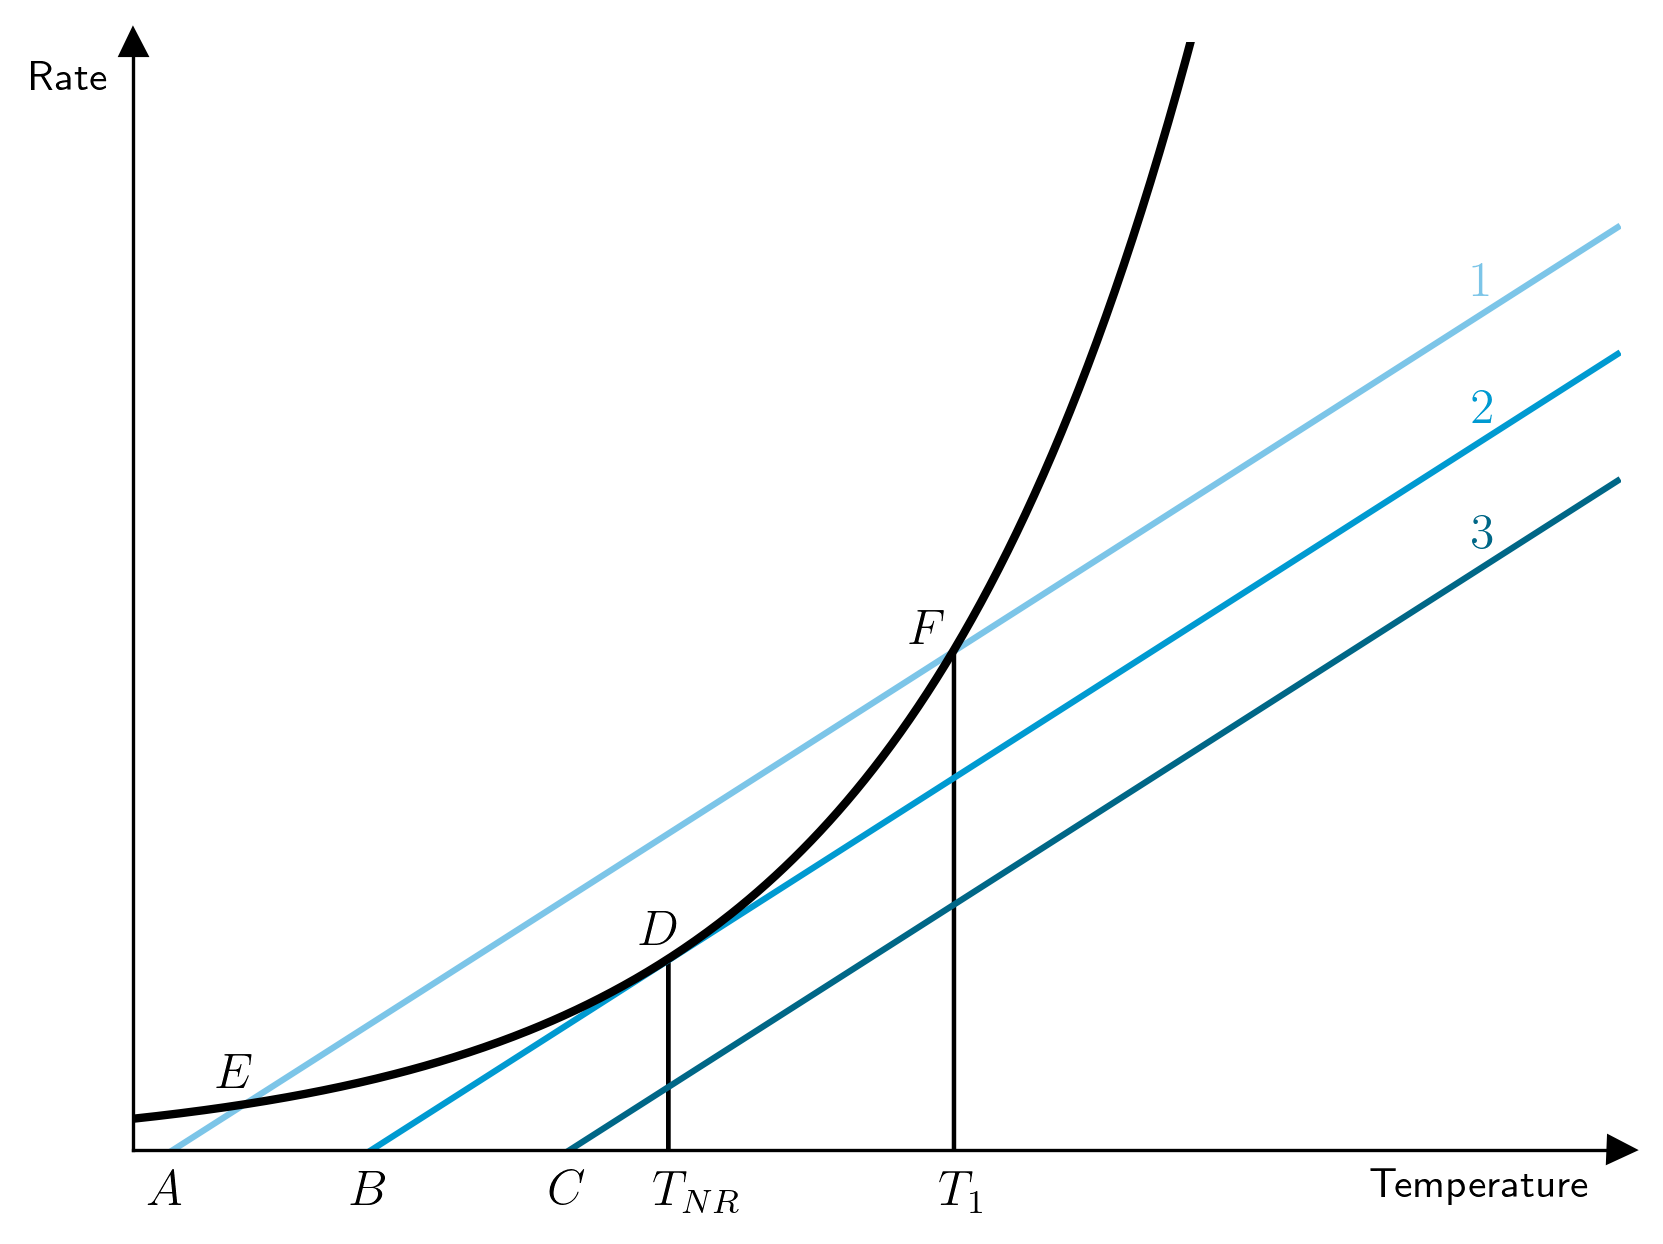
\includegraphics[width=0.7\textwidth]{Images/Chapter1/semenov-plot.png}
    \caption[Temperature dependence of reaction rate and heat loss]{Temperature dependence of reaction rate and heat loss from a system at three ambient temperature: $A$, $B$ and $C$. $A$ can control the sample temperature; $B$ is the critical temperature and the sample temperature can reach $T_{NR}$; if the ambient temperature exceeds $B$, the heat generation and losses are no longer balanced and the system will undergo thermal runaway. Source: Semenov (2013) \cite{semenov2013some}.}
    \label{fig:semenov-plot}
\end{figure}

Other info on thermal runaway can be found in "Thermal runaway - 2565" (in depth discussion), "Failure description - 43" (interesting perspective on the topic, it presents the failures per component with some nice graphs, in addition to in depth description of the reactions in thermal runaway), "Failure description - 890" (in depth discussion)

\section{Internal Short Circuit}
\label{sec:internal-short-circuit}

\section{Electric Failure and Abuse Testing}
\label{sec:electric-failure-abuse-testing}
Electric, Mechanical and Thermal failures can be found in "Safety Issues - 770"

\section{Mechanical Failure and Abuse Testing}
\label{sec:mechanical-failure-abuse-testing}

\section{Thermal Failure and Abuse Testing}
\label{sec:thermal-failure-abuse-testing}

\section{Safety Features in Commercial Batteries}
\label{sec:safety-features}
Can be found in "Safety Issues - 770", "Failure description - 43"

\section{CT for Degradation Studies}
\label{sec:ct-degradation-studies}